\documentclass[aspectratio=169,t]{beamer}

% ── PALETA EXACTA DEL MODELO ──────────────────────────────────────────────────
\usetheme{Madrid}
\usecolortheme{whale}

\definecolor{azuloscuro}{RGB}{25,25,89}
\definecolor{azulmedio}{RGB}{38,38,133}
\definecolor{azulclaro}{RGB}{214,214,239}

\setbeamercolor{palette primary}{bg=azuloscuro,fg=white}
\setbeamercolor{palette secondary}{bg=azulmedio,fg=white}
\setbeamercolor{palette tertiary}{bg=azuloscuro,fg=white}
\setbeamercolor{palette quaternary}{bg=azuloscuro,fg=white}
\setbeamercolor{structure}{fg=azuloscuro}
\setbeamercolor{frametitle}{bg=azuloscuro,fg=white}
\setbeamercolor{block title}{bg=azulmedio,fg=white}
\setbeamercolor{block body}{bg=white,fg=black}
\setbeamercolor{block title alerted}{bg=azuloscuro,fg=white}
\setbeamercolor{block body alerted}{bg=azulclaro!30,fg=black}
\setbeamercolor{block title example}{bg=azulmedio!80!black,fg=white}
\setbeamercolor{block body example}{bg=white,fg=black}
\setbeamercolor{item}{fg=azulmedio}
\setbeamercolor{section in toc}{fg=azuloscuro}

\setbeamerfont{frametitle}{size=\normalsize,series=\bfseries}
\setbeamerfont{block title}{size=\small,series=\bfseries}
\setbeamerfont{block title alerted}{size=\small,series=\bfseries}
\setbeamerfont{block title example}{size=\small,series=\bfseries}

% ── PAQUETES ──────────────────────────────────────────────────────────────────
\usepackage[spanish]{babel}
\usepackage[utf8]{inputenc}
\usepackage{amsmath,amssymb}
\usepackage{booktabs}
\usepackage{array}
\usepackage{colortbl}
\usepackage{graphicx}
\usepackage{tikz}
\usetikzlibrary{arrows.meta,positioning,shapes.geometric,calc}

% ── COMANDOS ──────────────────────────────────────────────────────────────────
\newcommand{\hl}[1]{\textcolor{azulmedio}{\textbf{#1}}}

% ── FOOTER ────────────────────────────────────────────────────────────────────
\setbeamertemplate{navigation symbols}{}
\setbeamertemplate{footline}{
  \leavevmode\hbox{%
    \begin{beamercolorbox}[wd=.42\paperwidth,ht=2.2ex,dp=1ex,center]{palette primary}
      \tiny Rond\'on
    \end{beamercolorbox}%
    \begin{beamercolorbox}[wd=.32\paperwidth,ht=2.2ex,dp=1ex,center]{palette secondary}
      \tiny Albertus (2019)
    \end{beamercolorbox}%
    \begin{beamercolorbox}[wd=.26\paperwidth,ht=2.2ex,dp=1ex,right]{palette primary}
      \tiny\insertframenumber/\inserttotalframenumber\hspace{1ex}
    \end{beamercolorbox}}
}

% ── METADATOS ─────────────────────────────────────────────────────────────────
\title[Land Reform \& Civil Conflict]{Land Reform and Civil Conflict: Theory and Evidence from Peru}
\subtitle{Albertus (2019) --- \textit{AJPS}}
\author[Rond\'on]{%
  Gabriel Rond\'on Quiroga (20212632) }
\institute[PUCP]{ECO25 --- Econometr\'ia Intermedia, PUCP}
\date{2025}

\begin{document}

%──────────────────────────────────────────────────────────────────────────────
% SLIDE 1 — PORTADA
%──────────────────────────────────────────────────────────────────────────────
{
\setbeamertemplate{footline}{}
\begin{frame}[plain]
\vspace{0.5cm}
\begin{center}
  {\color{azuloscuro}\rule{\textwidth}{2.5pt}}\vspace{0.3cm}

  {\Large\bfseries\color{azuloscuro}
    Land Reform and Civil Conflict:}\\[0.2cm]
  {\large\bfseries\color{azuloscuro}
    Theory and Evidence from Peru}\\[0.22cm]
  {\small\color{azulmedio}\textit{%
    Michael Albertus (2019) ---
    American Journal of Political Science}}

  \vspace{0.25cm}
  {\color{azuloscuro}\rule{\textwidth}{2.5pt}}
  \vspace{0.3cm}

  {\normalsize\color{azuloscuro}
    Gabriel Rond\'on Quiroga {\small(20212632)}
    $\;\cdot\;$
    Angelina Marzano {\small(20222890)}
    $\;\cdot\;$
    Joryeth Mar\'in }\\[0.18cm]
  {\small\color{gray}
    ECO25 --- Econometr\'ia Intermedia
    $\;|\;$ PUCP $\;|\;$ 2025}
\end{center}
\end{frame}
}

%──────────────────────────────────────────────────────────────────────────────
% SLIDE 2 — ÍNDICE
%──────────────────────────────────────────────────────────────────────────────
\begin{frame}{\'Indice}
  \tableofcontents
\end{frame}

%──────────────────────────────────────────────────────────────────────────────
% SLIDE 3 — INDICACIONES
%──────────────────────────────────────────────────────────────────────────────
\begin{frame}{Indicaciones}
\vspace{0.7cm}
\begin{itemize}\setlength{\itemsep}{0.55cm}
  \item El paper cuenta con replication files:
        \quad\hl{S\'i}~$\checkmark$
  \item El soporte visual del grupo ha sido elaborado
        en \LaTeX:\quad\hl{S\'i}~$\checkmark$
  \item El grupo ha efectuado an\'alisis adicionales
        con los datos del paper:\quad\hl{S\'i}~$\checkmark$
\end{itemize}
\end{frame}

%═════════════════════════════════════════════════════════════════════════════
\section{Introducci\'on}
%═════════════════════════════════════════════════════════════════════════════

%──────────────────────────────────────────────────────────────────────────────
% SLIDE 4 — INTRODUCCIÓN
%──────────────────────────────────────────────────────────────────────────────
\begin{frame}{Introducci\'on}
\begin{block}{Mensajes centrales del paper}
\small\begin{itemize}
  \item Reforma agraria de \hl{alta intensidad}
        $\Rightarrow$ \hl{reduce} el conflicto civil.
  \item Reforma agraria de \hl{baja intensidad}
        $\Rightarrow$ puede \hl{empeorarlo}.
  \item El v\'inculo pasa por relaciones organizativas
        Estado\,--\,civiles\,--\,guerrilla,
        no solo por agravios econ\'omicos.
\end{itemize}
\end{block}
\vspace{0.15cm}
\begin{columns}[T]
  \begin{column}{0.48\textwidth}
    \begin{alertblock}{La paradoja peruana}
    \small\begin{itemize}
      \item Reforma masiva (1969--1980):\\
            \hl{11 mill.\ ha},
            $\sim$21{,}000 expropiaciones
      \item Sendero Luminoso (1980--2000):\\
            \hl{$\sim$70{,}000 muertos} (CVR)
      \item Sendero naci\'o en \textbf{Ayacucho}
            --- zona de \hl{poca reforma}
    \end{itemize}
    \end{alertblock}
  \end{column}
  \begin{column}{0.48\textwidth}
    \begin{exampleblock}{Pregunta central}
    \small\textit{?`Es solo correlaci\'on, o la
    intensidad de la reforma causa m\'as o menos
    conflicto?}
    \vspace{0.15cm}

    \centering
    Reforma $\neq$ reducci\'on lineal\\[0.08cm]
    $\Downarrow$\\[0.05cm]
    \textbf{Relaci\'on en U invertida}
    \end{exampleblock}
  \end{column}
\end{columns}
\end{frame}

%──────────────────────────────────────────────────────────────────────────────
% SLIDE 5 — APORTES
%──────────────────────────────────────────────────────────────────────────────
\begin{frame}{Aportes del paper}
\begin{block}{Tres contribuciones principales}
\small\begin{enumerate}
  \item Estima el \hl{efecto causal} de la intensidad
        de la reforma sobre el conflicto a nivel de
        distrito --- no solo correlaci\'on.
  \item Identifica los \hl{cuatro mecanismos}:
        contrainsurgencia, organizaci\'on civil
        (rondas campesinas), competencia ideol\'ogica
        y costo de oportunidad.
  \item Evidencia para reformas \hl{top-down cl\'asicas}
        --- el 85\,\% de todas las grandes reformas desde
        1900, poco estudiadas con datos locales.
\end{enumerate}
\end{block}
\vspace{0.2cm}
\begin{alertblock}{?`Por qu\'e importa?}
\small La mayor\'ia de estudios previos usa datos
agregados nacionales. Este paper combina
\textbf{expropiaciones reales a nivel de distrito}
con \textbf{eventos de conflicto}, con un dise\~no
de identificaci\'on causal riguroso
(Fuzzy Geographic RDD).
\end{alertblock}
\end{frame}

%═════════════════════════════════════════════════════════════════════════════
\section{Objetivos}
%═════════════════════════════════════════════════════════════════════════════

%──────────────────────────────────────────────────────────────────────────────
% SLIDE 6 — PREGUNTA E HIPÓTESIS
%──────────────────────────────────────────────────────────────────────────────
\begin{frame}{Pregunta de investigaci\'on e hip\'otesis}
\begin{block}{Pregunta principal}
\small ?`C\'omo impacta la reforma agraria sobre la
intensidad del conflicto civil, y a trav\'es de
qu\'e mecanismos?
\end{block}
\vspace{0.1cm}
\begin{columns}[T]
  \begin{column}{0.50\textwidth}
    \begin{alertblock}{Hip\'otesis --- U invertida}
    \small\begin{itemize}
      \item \textbf{Sin reforma:} terratenientes controlan.
            Conflicto bajo por razones negativas.
      \item \textbf{Reforma baja:}
            \hl{m\'as conflicto}. Crea
            ganadores/perdedores, frustra expectativas.
      \item \textbf{Reforma alta:}
            \hl{menos conflicto}. Activa los cuatro
            mecanismos protectores.
    \end{itemize}
    \end{alertblock}
  \end{column}
  \begin{column}{0.46\textwidth}
  \centering\vspace{0.05cm}
  \begin{tikzpicture}[scale=0.78]
    \draw[->,thick,color=azuloscuro]
      (0,0)--(4.5,0)
      node[right,font=\small,color=azuloscuro]
        {\% Reforma};
    \draw[->,thick,color=azuloscuro]
      (0,0)--(0,3.0)
      node[above,font=\small,color=azuloscuro]
        {Conflicto};
    \draw[azulmedio,very thick,
          domain=0.1:4.3,samples=100]
      plot(\x,{2.5*\x*exp(-0.72*\x)+0.05});
    \draw[dashed,azulclaro!80]
      (1.39,0)--(1.39,2.2);
    \fill[azulmedio](1.39,2.2)circle(2.5pt);
    \node[above right,font=\tiny,color=azulmedio]
      at(1.39,2.2){inflexi\'on};
    \draw[azuloscuro,->,line width=1.2pt]
      (0.3,0.4)--(0.9,1.5)
      node[right,font=\tiny,color=azuloscuro]{$\uparrow$};
    \draw[azulmedio,->,line width=1.2pt]
      (1.8,1.85)--(3.1,0.45)
      node[right,font=\tiny,color=azulmedio]{$\downarrow$};
    \node[font=\tiny,color=azuloscuro]at(0.4,-0.28){baja};
    \node[font=\tiny,color=azuloscuro]at(3.2,-0.28){alta};
  \end{tikzpicture}
  \end{column}
\end{columns}
\end{frame}

%═════════════════════════════════════════════════════════════════════════════
\section{Literatura}
%═════════════════════════════════════════════════════════════════════════════

%──────────────────────────────────────────────────────────────────────────────
% SLIDE 7 — ESTADO DEL ARTE
%──────────────────────────────────────────────────────────────────────────────
\begin{frame}{Literatura relacionada: estado del arte}
\small
\begin{block}{Posici\'on 1 --- Reforma reduce conflicto}
Huntington (1968), Wood (2003). La tierra da algo que
perder $\Rightarrow$ reduce agravios y aumenta el costo
de oportunidad de rebelarse.
\end{block}
\vspace{0.09cm}
\begin{block}{Posici\'on 2 --- Evidencia mixta}
Albertus \& Kaplan (2013), Finkel et al.\ (2015).
El efecto depende del tipo de reforma, la represi\'on y
si los terratenientes capturan el proceso.
\end{block}
\vspace{0.09cm}
\begin{alertblock}{Posici\'on 3 --- Reforma parcial puede
    \hl{empeorar} el conflicto}
Albertus et al.\ (2018). Reformas de baja intensidad
crean ganadores/perdedores, frustran expectativas y
fracturan comunidades $\Rightarrow$ campo f\'ertil para
la insurgencia.
\end{alertblock}
\vspace{0.09cm}
\begin{exampleblock}{Literatura adicional}
\begin{itemize}
  \item Keele \& Titiunik (2015) ---
        Geographic RDD con fronteras administrativas.
  \item Dell (2010) ---
        Efectos persistentes de la mita colonial en Per\'u.
\end{itemize}
\end{exampleblock}
\end{frame}

%──────────────────────────────────────────────────────────────────────────────
% SLIDE 8 — APORTE DE ALBERTUS
%──────────────────────────────────────────────────────────────────────────────
\begin{frame}{Literatura relacionada: aporte de Albertus (2019)}
\begin{block}{Brecha que cubre este paper}
\small\begin{itemize}
  \item \textbf{Primer estudio} que combina expropiaciones
        reales a nivel de distrito con eventos de conflicto
        local para una reforma top-down cl\'asica.
  \item \textbf{Identifica mecanismos espec\'ificos} que
        conectan la reforma con el conflicto ---
        ausentes en estudios previos.
  \item \textbf{Dise\~no causal riguroso:}
        Fuzzy Geographic RDD con instrumento institucional.
\end{itemize}
\end{block}
\vspace{0.2cm}
\begin{columns}[T]
  \begin{column}{0.48\textwidth}
    \begin{alertblock}{\small Conexi\'on: RDD geogr\'afico}
    \small Keele \& Titiunik (2015) formalizan los supuestos
    del Geographic RDD, incluyendo el problema de
    \textbf{compound treatments} que Albertus aborda.
    \end{alertblock}
  \end{column}
  \begin{column}{0.48\textwidth}
    \begin{alertblock}{\small Conexi\'on: Per\'u}
    \small Dell (2010) documenta efectos persistentes
    de la mita colonial. Albertus la usa como
    covariable de control para absorber historia colonial.
    \end{alertblock}
  \end{column}
\end{columns}
\end{frame}

%═════════════════════════════════════════════════════════════════════════════
\section{Base de datos}
%═════════════════════════════════════════════════════════════════════════════

%──────────────────────────────────────────────────────────────────────────────
% SLIDE 9 — REFORMA Y CONFLICTO
%──────────────────────────────────────────────────────────────────────────────
\begin{frame}{Base de datos: reforma y conflicto}
\begin{columns}[T]
  \begin{column}{0.48\textwidth}
    \begin{block}{Tratamiento --- Reforma agraria}
    \small\begin{itemize}
      \item \textbf{Fuente:} \textit{El Peruano}, 1969--1980
      \item $\sim$21{,}000 expropiaciones individuales
      \item \textbf{Variable:} \% tierra del distrito
            redistribuida (0 a 1)
    \end{itemize}
    \end{block}
    \vspace{0.15cm}
    \begin{exampleblock}{\small
        Diferencia en el l\'imite ---
        1\textordfeminine\ etapa}
    \small\begin{itemize}
      \item N\'ucleo ($<$50 km): \hl{52.9\%}
      \item Periferia ($<$50 km): \hl{37.8\%}
      \item Diferencia:
            \hl{$\approx$\,+9.5 pp$^{**}$}
    \end{itemize}
    \end{exampleblock}
  \end{column}
  \begin{column}{0.48\textwidth}
    \begin{block}{Resultado --- Conflicto}
    \small\begin{itemize}
      \item \textbf{Fuente:} CVR (2004)
      \item \textbf{Var.\ 1:} total de ataques armados
            por distrito, 1980--2000
      \item \textbf{Var.\ 2:} total de muertes por
            distrito, 1980--2000
      \item \textbf{Var.\ 3:} control guerrillero ---
            distritos sin alcalde en 1989 o con
            $>$3 ataques en el per\'iodo
    \end{itemize}
    \end{block}
  \end{column}
\end{columns}
\end{frame}

%──────────────────────────────────────────────────────────────────────────────
% SLIDE 10 — CONTROLES Y DESCRIPTIVAS
%──────────────────────────────────────────────────────────────────────────────
\begin{frame}{Base de datos: controles y estad\'isticas descriptivas}
\begin{columns}[T]
  \begin{column}{0.36\textwidth}
    \begin{block}{Covariables de control}
    \scriptsize\begin{itemize}
      \item Poblaci\'on (censo 1972)
      \item Densidad de carreteras
      \item Personal del Estado (1961)
      \item Elevaci\'on y pendiente (FAO)
      \item \% tierra cultivable
      \item \'Area del distrito
      \item Zona mita (Dell 2010)
      \item Movimientos sociales previos
      \item \'Area privada (censo 1972)
      \item Coordenadas geogr\'aficas y
            efectos fijos de segmento
    \end{itemize}
    \end{block}
  \end{column}
  \begin{column}{0.61\textwidth}
    \begin{block}{Tabla 1 --- Estad\'isticas descriptivas}
    \scriptsize
    \begin{tabular}{lrrrr}
      \toprule
      \rowcolor{azuloscuro}
      \color{white}Variable &
      \color{white}Media &
      \color{white}D.E. &
      \color{white}M\'in &
      \color{white}M\'ax \\
      \midrule
      \rowcolor{azulclaro!60}
      Reforma (\%) & 0.14 & 0.24 & 0 & 1 \\
      Ataques & 7.82 & 37.87 & 0 & 661 \\
      \rowcolor{azulclaro!60}
      Muertes & 14.03 & 77.25 & 0 & 1{,}981 \\
      Poblaci\'on (miles) & 7.31 & 11.42 & 0.5 & 263 \\
      \rowcolor{azulclaro!60}
      Elevaci\'on (m) & 2{,}368 & 1{,}482 & 0 & 5{,}472 \\
      \bottomrule
      \multicolumn{5}{l}{\tiny
        $N=1{,}571$ distritos.
        Fuente: Tabla 1, Albertus (2019).}
    \end{tabular}
    \end{block}
    \vspace{0.1cm}
    \begin{alertblock}{\small Nota sobre la distribuci\'on}
    \small Ataques: media 7.82 pero D.E.\ 37.87 ---
    distribuci\'on muy asim\'etrica con muchos ceros.
    Justifica la \textbf{binomial negativa} en
    la Tabla 7.
    \end{alertblock}
  \end{column}
\end{columns}
\end{frame}

%═════════════════════════════════════════════════════════════════════════════
\section{Metodolog\'ia}
%═════════════════════════════════════════════════════════════════════════════

%──────────────────────────────────────────────────────────────────────────────
% SLIDE 11a — DAG: el diagrama (slide propio, centrado)
%──────────────────────────────────────────────────────────────────────────────
\begin{frame}{DAG: diagrama causal}
\vspace{0.2cm}
\begin{center}
\begin{tikzpicture}[
  every node/.style={font=\small},
  nodo/.style={
    rectangle, rounded corners=6pt,
    draw=azuloscuro, line width=1.6pt,
    fill=azulclaro!50,
    text width=2.8cm, align=center,
    minimum height=1.1cm},
  instr/.style={
    rectangle, rounded corners=6pt,
    draw=azulmedio, line width=2pt,
    fill=azulmedio!15,
    text width=2.8cm, align=center,
    minimum height=1.1cm},
  noobs/.style={
    ellipse,
    draw=azuloscuro, line width=1.4pt, dashed,
    fill=azulclaro!25,
    text width=2.5cm, align=center,
    minimum height=1.05cm},
  ->, >=Stealth,
  node distance=0.6cm and 2.6cm
]
  %% ── Nodos ─────────────────────────────────────────────────
  \node[instr](Z){
    \textbf{Zonas Agrarias}\\
    \textbf{1960 --- SIPA}\\[3pt]
    {\small\textit{Instrumento $C_i$}}};

  \node[nodo, right=2.5cm of Z](T){
    \textbf{\% Tierra}\\
    \textbf{redistribuida}\\[3pt]
    {\small\textit{Tratamiento $T_i$}}};

  \node[nodo, right=2.5cm of T](Y){
    \textbf{Conflicto}\\
    \textbf{1980--2000}\\[3pt]
    {\small\textit{Resultado $Y_i$}}};

  \node[noobs, above=1.3cm of T](U){
    \textbf{Caracts.}\\
    \textbf{previas $U$}\\[3pt]
    {\small\textit{No observable}}};

  %% ── Z → T: azulmedio sólido (1ª etapa) ───────────────────
  \draw[azulmedio, line width=2.2pt]
    (Z.east) -- (T.west);
  \node[font=\footnotesize, color=azulmedio,
        above=0.55cm of Z, xshift=1.85cm]
    {$\hat{\pi}_1 = 0.095^{**}$\;\; 1\textordfeminine\ etapa};

  %% ── T → Y: azuloscuro sólido (efecto causal) ─────────────
  \draw[azuloscuro, line width=2.2pt]
    (T.east) -- (Y.west);
  \node[font=\footnotesize, color=azuloscuro,
        above=0.55cm of T, xshift=1.85cm]
    {Efecto causal $\tau_{RD}$};

  %% ── U → T: azuloscuro punteado ───────────────────────────
  \draw[azuloscuro, dashed, line width=1.4pt, ->]
    (U.south west) -- (T.north);
  \node[font=\footnotesize, color=azuloscuro,
        left=0.1cm of T, yshift=1.4cm]
    {sesga $\hat{\beta}$};

  %% ── U → Y: azuloscuro punteado curvo ─────────────────────
  \draw[azuloscuro, dashed, line width=1.4pt, ->]
    (U.east) to[out=5, in=100, looseness=0.85] (Y.north);
  \node[font=\footnotesize, color=azuloscuro,
        right=0.1cm of T, yshift=1.4cm]
    {sesga $\hat{\beta}$};

  %% ── Z → Y: azulmedio punteado (restricción exclusión) ────
  \draw[azulmedio!60, dashed, line width=1.2pt, ->]
    (Z.south) to[out=-55, in=-125, looseness=0.5] (Y.south);
  \node[font=\footnotesize, color=azulmedio!80,
        below=1.25cm of T]
    {solo v\'ia $T_i$\;\; (restricci\'on de exclusi\'on)};

  %% ── Leyenda final ─────────────────────────────────────────
  \node[font=\small, color=azuloscuro, align=center,
        below=1.75cm of T]
    {\textbf{Backdoor path:}\;
     $U \to T_i$ y $U \to Y_i$
     $\Rightarrow$ sesga cualquier regresi\'on simple};
  \node[font=\small, color=azulmedio, align=center,
        below=2.2cm of T]
    {\textbf{El RDD cierra el backdoor
     autom\'aticamente al comparar en la frontera}};

\end{tikzpicture}
\end{center}
\end{frame}

%──────────────────────────────────────────────────────────────────────────────
% SLIDE 11b — DAG: la interpretación
%──────────────────────────────────────────────────────────────────────────────
\begin{frame}{DAG: interpretaci\'on del problema causal}
\vspace{0.1cm}
\begin{columns}[T]
  \begin{column}{0.32\textwidth}
    \begin{alertblock}{El problema}
    \small
    Regresar $Y_i$ sobre $T_i$ directamente
    sesga $\hat{\beta}$.\\[0.2cm]
    $U$ determina \textbf{tanto} la reforma
    \textbf{como} el conflicto --- abre un
    \textbf{backdoor path} que contamina
    el estimado.
    \end{alertblock}
  \end{column}
  \begin{column}{0.32\textwidth}
    \begin{block}{La soluci\'on}
    \small
    Distritos justo a cada lado del l\'imite
    son id\'enticos en $U$.\\[0.2cm]
    La \'unica diferencia es la intensidad
    de reforma --- determinada por criterios
    \textbf{agron\'omicos de 1960},
    no por $U$.\\[0.2cm]
    $\Rightarrow$ El RDD cierra el backdoor.
    \end{block}
  \end{column}
  \begin{column}{0.32\textwidth}
    \begin{block}{Restricci\'on de exclusi\'on}
    \small
    Las Zonas Agrarias ($C_i$) afectan el
    conflicto ($Y_i$)
    \textbf{solo a trav\'es de} la reforma
    ($T_i$).\\[0.2cm]
    No hay otro canal por el que cruzar
    el l\'imite nucleo/periferia afecte
    al conflicto.\\[0.2cm]
    An\'alogo al supuesto de exclusi\'on
    en variables instrumentales.
    \end{block}
  \end{column}
\end{columns}
\vspace{0.2cm}
\begin{alertblock}{}
\centering\small
\textbf{Leyenda del DAG:}\quad
{\color{azulmedio}$\longrightarrow$} Canal causal de inter\'es\quad
{\color{azuloscuro}$\cdots\!\to$} Backdoor path\quad
{\color{azulmedio!60}$\cdots\!\to$} Restricci\'on de exclusi\'on
\end{alertblock}
\end{frame}

%──────────────────────────────────────────────────────────────────────────────
% SLIDE 12 — ZONAS AGRARIAS
%──────────────────────────────────────────────────────────────────────────────
\begin{frame}{Estrategia de identificaci\'on --- Las Zonas Agrarias}
\begin{columns}[T]
  \begin{column}{0.54\textwidth}
    \begin{block}{El truco de identificaci\'on}
    \small\begin{enumerate}
      \item \textbf{1960:} SIPA crea 13 zonas por razones
            \hl{agron\'omicas} --- sin relaci\'on con
            pol\'itica redistributiva.
      \item \textbf{1969:} Velasco las usa por razones
            \hl{operativas} --- ya ten\'ian oficinas
            regionales activas.
      \item Departamento \textbf{n\'ucleo}: recibe
            \hl{mucha m\'as reforma}.
      \item Departamentos \textbf{perif\'ericos}
            adyacentes: reciben menos.
    \end{enumerate}
    \end{block}
    \vspace{0.1cm}
    \begin{exampleblock}{\small Variaci\'on cuasi-aleatoria}
    \small Nadie en 1960 pod\'ia saber que habr\'ia
    reforma en 1969. Los distritos
    \textbf{no pudieron elegir} su posici\'on.
    \end{exampleblock}
  \end{column}
  \begin{column}{0.43\textwidth}
    \begin{alertblock}{\small Ayacucho --- cuna de Sendero}
    \small Fragmentada entre zonas centradas en Ica,
    Huancavelica y Arequipa.
    \begin{itemize}
      \item[$\Rightarrow$]\hl{Poca reforma}
      \item[$\Rightarrow$]\hl{M\'as conflicto}
    \end{itemize}
    Consistente con la hip\'otesis.
    \end{alertblock}
    \vspace{0.15cm}
    \begin{block}{\small Diferencia en el l\'imite}
    \scriptsize
    \begin{tabular}{lc}
      \toprule
      \rowcolor{azuloscuro}
      \color{white}Grupo &
      \color{white}\% Reforma \\
      \midrule
      \rowcolor{azulclaro!60}
      N\'ucleo ($<$50 km) & \textbf{52.9\%}\\
      Periferia ($<$50 km) & \textbf{37.8\%}\\
      \midrule
      \rowcolor{azulclaro!30}
      \hl{Diferencia} &
      \hl{$\approx$ +9.5 pp$^{**}$}\\
      \bottomrule
    \end{tabular}
    \end{block}
  \end{column}
\end{columns}
\end{frame}

%──────────────────────────────────────────────────────────────────────────────
% SLIDE 13a — FUZZY RDD: Sharp vs Fuzzy
%──────────────────────────────────────────────────────────────────────────────
\begin{frame}{Dise\~no de investigaci\'on --- Sharp vs.\ Fuzzy RDD}
\vspace{-0.3cm}
\begin{columns}[T]

  \begin{column}{0.48\textwidth}
    \begin{block}{Sharp RDD (referencia)}
    \small
    El tratamiento pasa de 0 a 1
    \textbf{exactamente} en el cutoff:
    \[
      E[T_i \mid R_i = 0^{+}] = 1, \quad
      E[T_i \mid R_i = 0^{-}] = 0
    \]
    Se estima directamente con OLS.
    \end{block}
    \vspace{0.05cm}
    \begin{exampleblock}{Running variable y cutoff}
    \small
    \textbf{$R_i$}: distancia del centroide
    al l\'imite n\'ucleo/periferia (km)\\[0.08cm]
    $R_i > 0$: distrito n\'ucleo (tratado)\\
    $R_i < 0$: distrito perif\'erico (control)\\[0.08cm]
    \textbf{Cutoff = 0}: el l\'imite geogr\'afico exacto
    \end{exampleblock}
  \end{column}

  \begin{column}{0.48\textwidth}
    \begin{alertblock}{Fuzzy RDD --- nuestro caso}
    \small
    La probabilidad de reforma \textbf{salta}
    en el l\'imite, pero \textbf{no} de 0\,\% a 100\,\%:
    \[
      E[T_i \mid R_i = 0^{+}] > E[T_i \mid R_i = 0^{-}]
    \]
    \vspace{-0.3cm}
    \[
      \text{pero}\quad E[T_i \mid R_i = 0^{+}] < 1
    \]
    \vspace{-0.2cm}

    $\Rightarrow$ Se estima con \hl{2SLS}:
    $C_i$ (ser n\'ucleo) es el instrumento
    para $T_i$ (tierra redistribuida real).
    \end{alertblock}
    \vspace{0.05cm}
    \begin{block}{\small ?`Por qu\'e Fuzzy y no Sharp?}
    \small
    Algunos distritos perif\'ericos recibieron
    reforma; algunos n\'ucleos recibieron menos.
    La asignaci\'on no fue perfecta --- la
    probabilidad salta, no el tratamiento mismo.
    \end{block}
  \end{column}

\end{columns}
\end{frame}


\begin{frame}{Distribución de la Muestra}
    \begin{figure}
        \centering
        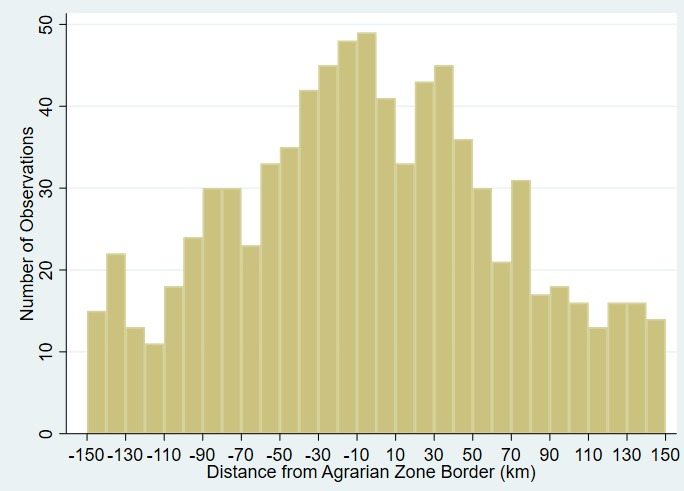
\includegraphics[width=0.5\linewidth]{images/WhatsApp Image 2026-06-05 at 10.46.46.jpeg}
        \caption{Distribución de las expropiaciones respecto a la distancia de la frontera}
    \end{figure}
    
\end{frame}


%──────────────────────────────────────────────────────────────────────────────
% SLIDE 13b — FUZZY RDD: el estimador LATE y detalles técnicos
%──────────────────────────────────────────────────────────────────────────────
\begin{frame}{Dise\~no de investigaci\'on --- El estimador LATE}
\vspace{0.1cm}
\begin{columns}[T]

  \begin{column}{0.54\textwidth}
    \begin{block}{El estimador LATE}
    \[
      \tau_{RD} \;=\;
      \frac{
        \displaystyle
        \lim_{r \to 0^{+}} E[Y_i \mid R_i = r]
        \;-\;
        \lim_{r \to 0^{-}} E[Y_i \mid R_i = r]
      }{
        \displaystyle
        \lim_{r \to 0^{+}} E[T_i \mid R_i = r]
        \;-\;
        \lim_{r \to 0^{-}} E[T_i \mid R_i = r]
      }
    \]
    \[
      = \;\frac{
          \text{Salto en } Y_i
          \;\text{(ITT)}
        }{
          \text{Salto en } T_i
          \;\text{(1\textordfeminine\ etapa)}
        }
    \]
    \small
    Identifica el efecto para distritos
    \textbf{en la frontera} (compliers).\\[0.1cm]
    El denominador escala el ITT por la fracci\'on
    de distritos que realmente cumpli\'o con el
    tratamiento.
    \end{block}
  \end{column}

  \begin{column}{0.43\textwidth}
    \begin{exampleblock}{Detalles t\'ecnicos}
    \small\begin{itemize}\setlength{\itemsep}{4pt}
      \item Kernel \textbf{triangular}:\\
            m\'as peso a observaciones
            cercanas al l\'imite
      \item Bandwidth \textbf{MSE-\'optimo}
            separado a cada lado\\
            (\texttt{bwselect(msetwo)})
      \item Errores clusterizados por
            \textbf{departamento}\\
            (\texttt{vce(nncluster depcode)})
      \item Regresi\'on local
            \textbf{lineal} (orden 1,
            \texttt{p(1)})
    \end{itemize}
    \end{exampleblock}
  \end{column}

\end{columns}
\end{frame}

%──────────────────────────────────────────────────────────────────────────────
% SLIDE 14 — ECUACIONES (corregidas y bien escritas)
%──────────────────────────────────────────────────────────────────────────────
\begin{frame}{Ecuaciones del modelo}

  \begin{block}{Primera etapa ---
      Efecto del instrumento sobre el tratamiento}
  \[
    T_i \;=\; \pi_0
            + \pi_1 C_i
            + \pi_2 R_i
            + \pi_3 (R_i \times C_i)
            + \mathbf{X}_i'\,\delta
            + u_i
    \qquad
    \hat{\pi}_1 \approx +0.095^{**}
  \]
  \end{block}

  \vspace{0.15cm}

  \begin{block}{Segunda etapa ---
      Efecto causal sobre el conflicto}
  \[
    Y_i \;=\; \alpha
            + \tau_{RD}\,\hat{T}_i
            + \beta_1 R_i
            + \beta_2 C_i
            + \beta_3 (R_i \times C_i)
            + \mathbf{X}_i'\,\gamma
            + \varepsilon_i
  \]
  \end{block}

  \vspace{0.18cm}

  \scriptsize
  \centering
  \begin{tabular}{clcl}
    \toprule
    \rowcolor{azuloscuro}
    \color{white}S\'imbolo &
    \color{white}Definici\'on &
    \color{white}S\'imbolo &
    \color{white}Definici\'on \\
    \midrule
    \rowcolor{azulclaro!50}
    $Y_i$ & Total ataques o muertes, 1980--2000 &
    $T_i$ & \% tierra redistribuida \\
    $\hat{T}_i$ & $T_i$ predicho --- elimina endogeneidad &
    $R_i$ & Distancia al l\'imite (km) \\
    \rowcolor{azulclaro!50}
    $C_i$ & $=1$ si n\'ucleo (instrumento) &
    $\tau_{RD}$ & \textbf{LATE --- efecto causal} \\
    $\mathbf{X}_i$ & Covariables de control &
    $\pi_1$ & Fuerza de la 1\textordfeminine\ etapa \\
    \bottomrule
  \end{tabular}

\end{frame}

\begin{frame}{RD 1era etapa}
    \begin{figure}
        \centering
        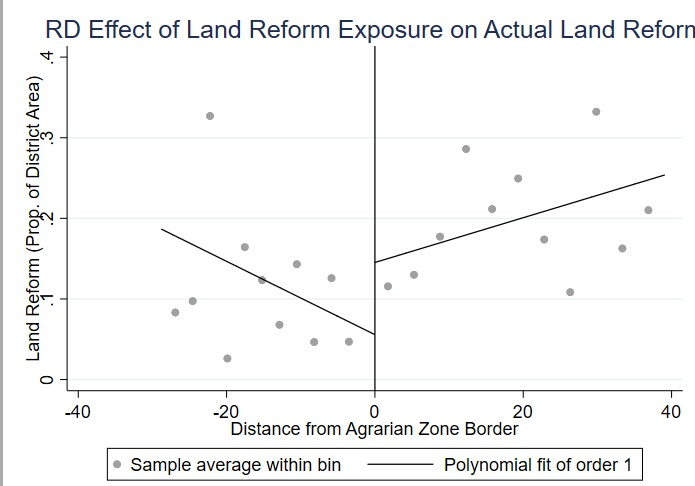
\includegraphics[width=0.5\linewidth]{images/WhatsApp Image 2026-06-05 at 10.57.58.jpeg}
        \caption{Enter Caption}
        
    \end{figure}
    Efecto de la distancia a la frontera sobre la tierra redistribuida
\end{frame}


%──────────────────────────────────────────────────────────────────────────────
% SLIDE 15 — SUPUESTOS
%──────────────────────────────────────────────────────────────────────────────
\begin{frame}{Supuestos de identificaci\'on}
\scriptsize
\begin{tabular}{>{\bfseries\small}p{4cm}
                p{3.4cm} p{4.5cm}}
  \toprule
  \rowcolor{azuloscuro}
  \color{white}Supuesto &
  \color{white}?`Qu\'e implica? &
  \color{white}?`C\'omo lo defiende Albertus? \\
  \midrule
  \rowcolor{azulclaro!50}
  1. Continuidad &
  Sin tratamiento, no habr\'ia salto en conflicto
  al cruzar el l\'imite &
  Balance de 11 covariables
  pre-reforma como outcome. Ninguna salta
  (solo pendiente, controlada directamente) \\
  \midrule
  2. No manipulaci\'on &
  Los distritos no pudieron elegir estar en
  n\'ucleo o periferia &
  Zonas creadas en 1960 por razones agron\'omicas,
  10 a\~nos antes de la reforma.
  Test de McCrary: sin bunching \\
  \midrule
  \rowcolor{azulclaro!50}
  3. Compound Treatment Irrelevance &
  Solo la reforma cambia relevantemente
  al cruzar el l\'imite departamental &
  Per\'u: Estado unitario centralizado.
  \textbf{Tablas A2 y A3:} balance en capacidad
  estatal y escolaridad. Todos no significativos \\
  \midrule
  4. LATE interpretable &
  El efecto en el margen es relevante
  para la teor\'ia &
  La teor\'ia predice efecto al comparar
  alta vs.\ baja reforma --- exactamente
  lo que var\'ia en la frontera \\
  \bottomrule
\end{tabular}
\end{frame}

%──────────────────────────────────────────────────────────────────────────────
% SLIDE 16 — LIMITACIONES
%──────────────────────────────────────────────────────────────────────────────
\begin{frame}{Limitaciones del m\'etodo}
\begin{columns}[T]
  \begin{column}{0.48\textwidth}
    \begin{alertblock}{Limitaciones de dise\~no}
    \small\begin{itemize}
      \item \textbf{Validez externa limitada:}
            el LATE aplica solo a distritos en la
            frontera --- no extrapolable a todo
            Per\'u ni a otros pa\'ises
      \item \textbf{Compound treatment:}
            an\'alogo a la restricci\'on de exclusi\'on
            en IV --- no completamente verificable
      \item \textbf{Spillovers:} ?`el conflicto
            se desplaz\'o a distritos adyacentes?
    \end{itemize}
    \end{alertblock}
  \end{column}
  \begin{column}{0.48\textwidth}
    \begin{alertblock}{Limitaciones de datos y teor\'ia}
    \small\begin{itemize}
      \item \textbf{Subregistro CVR:}
            alta represi\'on $\Rightarrow$ miedo a
            testificar $\Rightarrow$ conflicto
            subestimado donde fue m\'as intenso
      \item \textbf{Mecanismos sugerentes:}
            tests de la Tabla 6 no est\'an
            causalmente identificados
      \item \textbf{Reforma interrumpida:}
            se detuvo en 1976 antes de completarse
            por la crisis econ\'omica
    \end{itemize}
    \end{alertblock}
  \end{column}
\end{columns}
\end{frame}

%------- Sección de Resultados ----------------
\section{Resultados}

%------ Diapo Efectos de la reforma-----
\begin{frame}{Efectos de la reforma}
    \begin{table}[h]
\centering
\caption{RD Effect of Land Reform on Total Conflict Events}
\label{tab:rd_results}
\small
\resizebox{\textwidth}{!}{
\begin{tabular}{lccccc}
\toprule
& \textbf{Prop. land area} & \textbf{Prop. land area} & \textbf{Prop. land area} & \textbf{Prop. land area} & \textbf{Prop. land area} \\
\textbf{Land reform measure:} & \textbf{redistributed} & \textbf{redistributed} & \textbf{redistributed} & \textbf{redistributed} & \textbf{redistributed} \\
\cmidrule(lr){2-6}
& \textbf{Total} & \textbf{Total} & \textbf{Conflict} & \textbf{Guerrilla control} & \textbf{Guerrilla control} \\
\textbf{Dependent variable:} & \textbf{attacks} & \textbf{attacks} & \textbf{deaths} & \textbf{(no mayor in 1989)} & \textbf{($>$3 attacks)} \\
\midrule
Treatment Effect Estimate
    & $-11.704^{**}$ & $-12.176^{**}$ & $-35.598^{**}$ & $-1.759^{*}$  & $-0.456^{*}$  \\
    & $(0.043)$      & $(0.011)$      & $(0.032)$      & $(0.084)$     & $(0.085)$     \\[4pt]
First-Stage Estimate
    & $0.095^{**}$   & $0.102^{***}$  & $0.104^{***}$  & $0.111^{***}$ & $0.096^{***}$ \\
    & $(0.020)$      & $(0.002)$      & $(0.001)$      & $(0.001)$     & $(0.006)$     \\[4pt]
Bandwidth {[}Left, Right{]}
    & {[}34.45, 39.82{]} & {[}33.32, 47.48{]} & {[}31.05, 44.43{]} & {[}34.10, 68.28{]} & {[}35.86, 51.03{]} \\[2pt]
Treated Observations
    & 161 & 192 & 177 & 247 & 203 \\
Control Observations
    & 161 & 154 & 144 & 157 & 162 \\
Geographic Controls
    & Yes & Yes & Yes & Yes & Yes \\
Includes Covariates
    & No  & Yes & Yes & Yes & Yes \\
\bottomrule
\end{tabular}
}
\end{table}
\end{frame}

\begin{frame}{Regresión discontinua 2da etapa}
    \begin{figure}
        \centering
        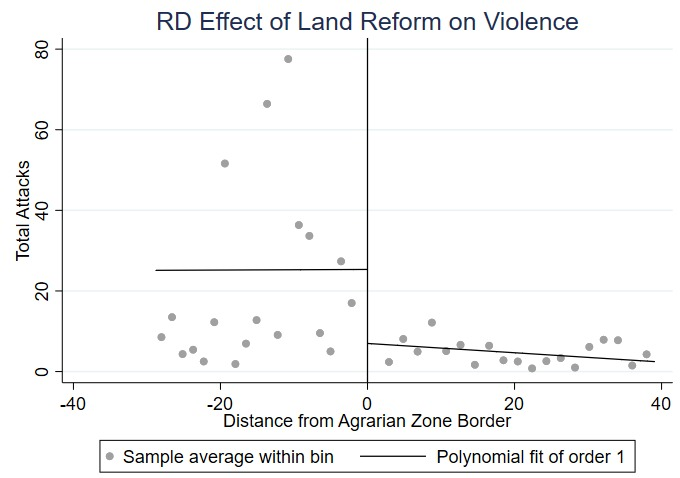
\includegraphics[width=0.5\linewidth]{images/WhatsApp Image 2026-06-05 at 10.46.49.jpeg}
        \caption{Representación gráfica del efecto causal de la reforma agraria sobre la violencia política}
        \label{Ataques con respecto de la distancia con la frontera}
    \end{figure}
\end{frame}



%---------------Diapo Validez----------------
\begin{frame}{Validez}
  
\begin{table}[h]
    \centering
    \caption{Balance de covariables}
    \label{tab:placeholder_label}
    \begin{tabular}{lcccccc}
        \toprule
        & \multicolumn{1}{c}{Estimated} & & \multicolumn{1}{c}{Bandwidth} & \multicolumn{1}{c}{Treated} & \multicolumn{1}{c}{Control} \\
        & \multicolumn{1}{c}{Difference} & \multicolumn{1}{c}{p-value} & \multicolumn{1}{c}{[Left, Right]} & \multicolumn{1}{c}{Obs.} & \multicolumn{1}{c}{Obs.} \\
        \midrule
        Population            &  1.71  & 0.50 & [64.33, 49.69]  & 198 & 259 \\
        Road density          &  0.26  & 0.77 & [35.81, 41.30]  & 166 & 162 \\
        State personnel       & $-0.04$ & 0.69 & [60.49, 64.29]  & 235 & 253 \\
        Elevation             & $-0.53$ & 0.23 & [60.87, 48.35]  & 196 & 253 \\
        Slope                 & $-2.76^{**}$ & 0.01 & [25.16, 41.85]  & 168 & 121 \\
        Cultivable land       & $-0.48$ & 0.35 & [38.90, 38.93]  & 158 & 179 \\
        District area         &  0.59  & 0.55 & [35.74, 37.16]  & 149 & 162 \\
        Mita zone             & $-0.39$ & 0.14 & [109.31, 72.09] & 258 & 375 \\
        Prior social movements&  0.04  & 0.18 & [27.48, 23.81]  &  90 & 132 \\
        Private land area     & 16.00  & 0.23 & [43.32, 158.43] & 401 & 193 \\
        \bottomrule
    \end{tabular}
\end{table}
\end{frame}


%-----------Pruebas placebo--------------------
\begin{frame}{Pruebas placebo}
\vfill
\begin{center}
Cuadro: Placebo tests
\resizebox{\textwidth}{!}{%
\small
\begin{tabular}{lcccccccccc}
\toprule
& \textbf{15 km} & \textbf{5 km} & \textbf{2 km} & \textbf{True} & \textbf{2 km} & \textbf{5 km} & \textbf{15 km} & \textbf{Land Reform} & \textbf{Ag. Zone 2} \\
& \textbf{Outside} & \textbf{Outside} & \textbf{Outside} & \textbf{Boundary} & \textbf{Inside} & \textbf{Inside} & \textbf{Inside} & \textbf{Treatment:} & \textbf{Periph/Periph} \\
& & & & & & & & \textbf{Uncult. Land} & \textbf{Boundary} \\
\midrule
Treatment Effect    & $-4.433$      & $15.942$      & $-15.518^{**}$ & $-12.176^{**}$ & $-9.261^{**}$ & $-3.651$      & $113.800$     & $784.56$      & $178.42$      \\
Estimate            & $(0.230)$     & $(0.408)$     & $(0.037)$      & $(0.011)$      & $(0.010)$     & $(0.375)$     & $(0.821)$     & $(0.900)$     & $(0.868)$     \\[4pt]
First-Stage         & $-0.092^{**}$ & $-0.044$      & $0.072^{*}$    & $0.102^{***}$  & $0.123^{***}$ & $0.143^{***}$ & $0.004$       & $-0.002$      & $0.004$       \\
Estimate            & $(0.035)$     & $(0.284)$     & $(0.050)$      & $(0.002)$      & $(0.000)$     & $(0.000)$     & $(0.896)$     & $(0.182)$     & $(0.912)$     \\[4pt]
Bandwidth (Left)    & 55.03  & 51.15  & 37.04  & 33.32  & 32.50  & 32.52  & 44.65  & 26.28  & 30.43  \\
Bandwidth (Right)   & 49.74  & 44.99  & 46.90  & 47.48  & 49.74  & 66.87  & 51.44  & 44.87  & 28.51  \\
Treated Obs.        & 209    & 177    & 177    & 192    & 207    & 244    & 183    & 177    & 29     \\
Control Obs.        & 206    & 219    & 180    & 154    & 142    & 143    & 195    & 123    & 34     \\
\bottomrule
\end{tabular}
}
\end{center}
\vfill
\end{frame}

%% ── Diapositiva 1: Paneles A y B ──────────────────────
\begin{frame}{Tabla 6: Mecanismos (1/2)}
\vspace{-0.5cm}
\begin{center}
\begin{table}
    \resizebox{\textwidth}{!}{%
    \small
    \begin{tabular}{lcccccc}
    \toprule
    \textbf{Dependent Variable}
        & \textbf{Treatment}  & \textbf{First-Stage} & \textbf{Bandwidth} & \textbf{Bandwidth} & \textbf{Treated} & \textbf{Control} \\
        & \textbf{Effect Est.}& \textbf{Estimate}    & \textbf{(Left)}    & \textbf{(Right)}   & \textbf{Obs.}    & \textbf{Obs.}    \\
    \midrule
    \multicolumn{7}{l}{\textbf{Panel A: Counterinsurgency and Government Strategy}} \\
    \midrule
    Deaths from Guerrilla Forces, 1980--1988
        & $-10.156^{*}$  & $0.105^{***}$ & 31.74 & 55.53 & 215 & 147 \\
        & $(0.064)$      & $(0.000)$     &       &       &     &     \\[0.5pt]
    Deaths from Guerrilla Forces, 1989--2000
        & $-4.246^{**}$  & $0.095^{***}$ & 36.17 & 51.37 & 205 & 164 \\
        & $(0.031)$      & $(0.006)$     &       &       &     &     \\[0.5pt]
    Deaths from State Forces, 1980--1988
        & $-2.042$       & $0.086^{**}$  & 39.32 & 54.53 & 212 & 181 \\
        & $(0.527)$      & $(0.011)$     &       &       &     &     \\[0.5pt]
    Deaths from State Forces, 1989--2000
        & $-11.010^{**}$ & $0.120^{***}$ & 31.66 & 74.64 & 265 & 146 \\
        & $(0.010)$      & $(0.000)$     &       &       &     &     \\[0.5pt]
    Emergency Zone Declaration
        & $-2.191^{**}$  & $0.106^{***}$ & 21.03 & 49.30 & 164 & 85  \\
        & $(0.037)$      & $(0.002)$     &       &       &     &     \\
    \midrule
    \multicolumn{7}{l}{\textbf{Panel B: Civilian Organization}} \\
    \midrule
    Participation in \textit{Ronda Campesina}
        & $1.070^{**}$   & $0.096^{***}$ & 33.55 & 39.34 & 157 & 156 \\
        & $(0.046)$      & $(0.005)$     &       &       &     &     \\[0.5pt]
    Participation in Producer Organization
        & $-0.462$       & $0.076^{*}$   & 40.94 & 40.25 & 161 & 186 \\
        & $(0.289)$      & $(0.078)$     &       &       &     &     \\
    \bottomrule
    \end{tabular}
    }
\end{table}
\end{center}

\end{frame}

%% ── Diapositiva 2: Paneles C y D ──────────────────────
\begin{frame}{Mecanismos (2/2)}
\vfill
\begin{center}
\begin{table}
    \resizebox{\textwidth}{!}{%
    \small
    \begin{tabular}{lcccccc}
    \toprule
    \textbf{Dependent Variable}
        & \textbf{Treatment}  & \textbf{First-Stage} & \textbf{Bandwidth} & \textbf{Bandwidth} & \textbf{Treated} & \textbf{Control} \\
        & \textbf{Effect Est.}& \textbf{Estimate}    & \textbf{(Left)}    & \textbf{(Right)}   & \textbf{Obs.}    & \textbf{Obs.}    \\
    \midrule
    \multicolumn{7}{l}{\textbf{Panel C: Ideological Competition}} \\
    \midrule
    Marxist Vote, 1980
        & $-0.316^{*}$   & $0.103^{***}$ & 36.34 & 65.71 & 237 & 164 \\
        & $(0.092)$      & $(0.000)$     &       &       &     &     \\
    \midrule
    \multicolumn{7}{l}{\textbf{Panel D: Opportunity Costs}} \\
    \midrule
    Total Attacks in Districts Higher than 1500m
        & $-14.339^{**}$ & $0.122^{***}$ & 28.36 & 35.26 & 91  & 121 \\
        & $(0.011)$      & $(0.002)$     &       &       &     &     \\[3pt]
    Total Attacks in Districts Higher than 2500m
        & $-16.015^{**}$ & $0.120^{**}$  & 21.97 & 48.29 & 108 & 81  \\
        & $(0.025)$      & $(0.032)$     &       &       &     &     \\
    \bottomrule
    \end{tabular}
    }
\end{table}
\end{center}
\vfill
\end{frame}


%Análisis adicional
\begin{frame}{Análisis adicional: U invertida (Binomial Negativa, N = 1,445)}

\begin{columns}[c]

\column{0.58\textwidth}
\centering

\begin{figure}
    \centering
    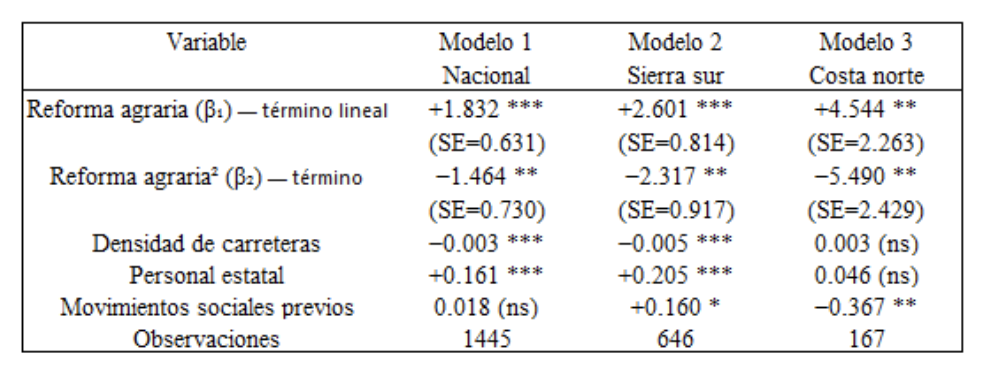
\includegraphics[width=1\linewidth]{images/image.png}
    
\end{figure}
\column{0.35\textwidth}

\small

El punto de inflexión se calcula como:

\[
D^*=\frac{\beta_1}{2\times|\beta_2|}
\]

En la costa el punto llega antes (41\%) porque la reforma costera creó cooperativas exportadoras muy rentables. Los campesinos tenían más que perder apoyando a Sendero.

\vspace{0.2cm}

Ayacucho recibió poca reforma y se ubicó en el tramo ascendente de la curva, donde se observa el máximo nivel de conflicto.

\end{columns}
\end{frame}

\begin{frame}{Gráfico:  Curva de U invertida (Tabla 7, con datos reales)}

\begin{figure}
    \centering
    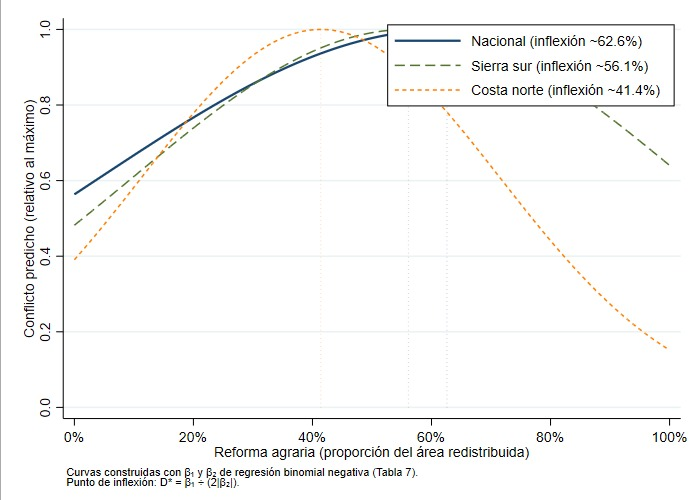
\includegraphics[width=0.5\linewidth]{images/WhatsApp Image 2026-06-05 at 10.46.39.jpeg}
    \caption{Los puntos de inflexión identifican el umbral en el que la reforma agraria deja de incrementar el conflicto y comienza a reducirlo}
\end{figure}

\end{frame}

%------------Conclusión-----------------------
\section{Conclusión}
\begin{frame}{Conclusión}
  La reforma agraria ha tenido efectos sobre el levantamiento de movimientos como Sendero Luminoso:
  \begin{itemize}
      \item La reforma afectó la organización civil, la cual fue fundamental en la lucha contra las guerrillas
      \item Una implementación parcial de la reforma generó un levantamiento pronunciado por parte de grupos armados
      \item Una implementación más intensa mitiga los efectos
      \item Los distritos que son periféricos han sufrido un mayor efecto por parte de grupos como Sendero Luminoso
  \end{itemize}
  Este estudio permite comprender la dinámica de conflictos armados entre pobladores rurales, insurgentes y el estado en otros países donde la reforma agraria ha coincidido con un posterior conflicto rural
\end{frame}



\end{document}
